\documentclass[11pt]{article}
\usepackage[margin=1in]{geometry}
\usepackage[T1]{fontenc}
\usepackage{lmodern}
\usepackage{amsmath,amssymb,amsthm,bm}
\usepackage{booktabs,graphicx,caption,subcaption}
\usepackage[authoryear,round]{natbib}
\usepackage[hidelinks]{hyperref}
\usepackage{xcolor}
\usepackage{setspace}
\onehalfspacing

\newtheorem{proposition}{Proposition}
\newtheorem{lemma}{Lemma}
\newtheorem{definition}{Definition}
\theoremstyle{remark}
\newtheorem{remark}{Remark}

\newcommand{\1}{\mathbf{1}}
\newcommand{\E}{\mathbb{E}}
\newcommand{\F}{\mathcal{F}}
\newcommand{\VaR}{\mathrm{VaR}}
\newcommand{\ES}{\mathrm{ES}}
\newcommand{\todo}[1]{\textcolor{red}{[TODO: #1]}}

\title{Learning the Tail: Deep Joint Forecasting of Value-at-Risk and Expected Shortfall with Strictly Consistent Scoring Functions}
\author{Mayur Agrawal\thanks{Department of Computer Science and Engineering and Department of Economic Sciences, Indian Institute of Technology Kanpur, Kanpur 208016, India. Email: \href{mailto:mayurag22@iitk.ac.in}{mayurag22@iitk.ac.in}. Code and data pipeline: \url{https://github.com/mayur-agrawal-iitk/learning-the-tail}.}}
\date{\today}

\begin{document}
\maketitle

\begin{abstract}
Expected Shortfall (ES), the market-risk measure of the Basel framework, is not elicitable on its own, but it is jointly elicitable with Value-at-Risk (VaR). We use this fact to train deep sequence models directly on a strictly consistent scoring function for (VaR, ES), the FZ0 loss. We prove that pooling across assets on volatility-standardised returns is exactly equivalent to training on raw returns. We also design an output layer that rules out crossing risk forecasts by construction. In a twenty-year out-of-sample study of twelve global equity indices at the 1\%, 2.5\% and 5\% levels, we compare an LSTM, a Transformer and a GARCH--LSTM hybrid with nine benchmarks, including GARCH-EVT, filtered historical simulation and score-driven FZ-GAS models. A pooled LSTM that sees only past returns is statistically indistinguishable from the best econometric models and is the only single model in every model confidence set. The deep models are, moreover, complementary to the econometric ones. Adding them to an equal-weight combination of the econometric models lowers the FZ0 loss at every risk level (Diebold--Mariano $t$ between $-4.7$ and $-5.3$; significant in 10--11 of 12 markets, never significantly worse). The resulting combination is the best model overall and requires about 2\% less capital than GJR-GARCH with the same Basel traffic-light record. The deep models' weaknesses are calibration and sudden volatility spikes such as March 2020.

\end{abstract}

\noindent\textbf{Keywords:} Expected Shortfall, Value-at-Risk, elicitability, deep learning, LSTM, GARCH, extreme value theory, forecast evaluation.\\
\noindent\textbf{JEL:} C22, C45, C52, C53, G17, G32.

%==============================================================================
\section{Introduction}\label{sec:intro}
%==============================================================================

Since the Fundamental Review of the Trading Book, the Basel framework measures market risk with the 97.5\% Expected Shortfall (ES) rather than the 99\% Value-at-Risk (VaR) \citep{bcbs2019frtb}. ES is coherent \citep{artzner1999coherent} and, unlike VaR, it is sensitive to the size of losses beyond the quantile. Forecasting ES, however, raises a statistical problem that VaR does not: ES is not \emph{elicitable} \citep{gneiting2011making}. There is no loss function whose expected value is minimised by the true ES, so ES forecasts cannot be estimated or ranked by minimising an average loss in the way that quantiles are with the pinball loss. \citet{fissler2016higher} showed that the \emph{pair} (VaR, ES) is jointly elicitable and characterised the class of strictly consistent scoring functions for it. \citet{patton2019dynamic} then used one member of that class, the FZ0 loss, to estimate semiparametric dynamic models for VaR and ES.

The same result has a direct implication for machine learning that has been less explored. A strictly consistent scoring function is exactly what is needed to train a flexible function approximator by empirical risk minimisation. A neural network trained on the FZ0 loss is a nonparametric M-estimator of the conditional (VaR, ES) pair. It needs no distributional assumption and no separate quantile and tail-mean steps. This paper asks a simple question: \emph{once evaluated with a strictly consistent scoring function and the standard battery of regulatory backtests, do deep sequence models forecast tail risk better than state-of-the-art econometric models?}

We answer it with a large, carefully controlled out-of-sample experiment. We forecast one-day-ahead VaR and ES at $\alpha\in\{1\%,2.5\%,5\%\}$ for twelve equity indices from developed and emerging markets over 2006--2026. This period contains the global financial crisis, the euro-area crisis, the COVID-19 crash and the 2022 inflation shock. We compare three deep models with nine benchmarks. The benchmarks span the three main approaches in the literature: parametric location-scale models (GARCH, GJR-GARCH with Student-$t$ and skewed-$t$ innovations), semi-parametric tail estimators (filtered historical simulation, GARCH-EVT), and dynamic semiparametric models estimated by FZ0 minimisation (CAViaR-ES, FZ-GAS and its hybrid). All models use the same information set (past daily returns only) and the same rolling estimation window.

\paragraph{Contributions.}
\begin{enumerate}
\item \emph{Methodology.} We show how to train deep networks directly on the FZ0 loss and pool data across assets. We prove that, because FZ0 loss differences are invariant to scale, training on volatility-standardised returns is exactly equivalent to training on raw returns (Proposition~\ref{prop:scale}). We also design an output layer that guarantees $\ES_t\le\VaR_t<0$ and non-crossing across risk levels by construction (Proposition~\ref{prop:head}).
\item \emph{A hybrid model.} We propose a GJR-GARCH--LSTM hybrid in which the GARCH filter handles the volatility scale and the network learns a time-varying conditional \emph{tail shape}. This nonparametric counterpart of autoregressive conditional density models \citep{hansen1994autoregressive} is interpretable through the implied ES/VaR ratio.
\item \emph{Evidence.} We provide a comprehensive evaluation that combines absolute tests (coverage, independence, dynamic-quantile and three ES backtests) with relative tests (panel Diebold--Mariano and the Model Confidence Set). The evaluation includes crisis subperiods, seed-ensemble robustness and pre-specified forecast combinations. The main finding is that deep models trained on FZ0 match the best econometric models and are complementary to them.
\end{enumerate}

\paragraph{Preview of results.} A pooled LSTM that sees only past returns is statistically indistinguishable from GJR-GARCH with skewed-$t$ innovations, filtered historical simulation and GARCH-EVT, the best econometric models. It is the only single model in the 90\% model confidence set for all 36 market--risk-level combinations. Adding the three deep models to an equal-weight combination of the econometric models significantly lowers the FZ0 loss at every risk level (panel Diebold--Mariano $t$ between $-4.7$ and $-5.3$). The gain is significant in 10 or 11 of 12 markets and accumulates steadily over twenty years. That combination is the best model in the study. At the same Basel traffic-light record it requires about 2\% less capital than GJR-GARCH. The deep models' weaknesses are interpretable: they are slightly less conservative than the best econometric models, and they adapt more slowly to sudden volatility spikes such as March 2020. The score-driven FZ-GAS models of \citet{patton2019dynamic} underperform in our sample, even with a carefully verified estimator.

%==============================================================================
\section{Related literature}\label{sec:lit}
%==============================================================================

\paragraph{Elicitability and ES.} \citet{gneiting2011making} showed that ES fails the convex-level-set condition necessary for elicitability. \citet{fissler2016higher} established joint elicitability of (VaR, ES), and \citet{nolde2017elicitability} drew out the implications for backtesting and regulation. They distinguish \emph{comparative} backtests based on consistent scores from traditional \emph{calibration} tests. \citet{ziegel2020robust} study how rankings depend on the choice of scoring function within the consistent class.

\paragraph{Econometric models for VaR and ES.} Location-scale models with GARCH-type volatility \citep{bollerslev1986garch,glosten1993relation} and flexible innovation densities \citep{hansen1994autoregressive} remain the industry workhorse. Filtered historical simulation \citep{baroneadesi1999var} and the GARCH-EVT approach of \citet{mcneil2000estimation} replace the parametric innovation tail by an empirical or generalised Pareto tail. Quantile-based models model VaR dynamics directly \citep{engle2004caviar} and were extended to ES by \citet{taylor2019forecasting} and \citet{patton2019dynamic}. The latter introduced score-driven \citep{creal2013generalized} dynamics derived from the FZ0 loss.

\paragraph{Machine learning for risk.} Neural networks were used early for quantile forecasting \citep{taylor2000quantile}. More recent studies find gains from machine learning for volatility forecasting \citep{bucci2020realized,christensen2023machine} and for return prediction \citep{gu2020empirical}. For tail risk specifically, \citet{li2021bayesian} embed an LSTM in an ES-CAViaR model estimated by Bayesian MCMC. \citet{stateful2024rnn} propose recurrent-network-based stateful models for joint VaR and ES forecasting. \citet{zhang2026resga} train a large cross-sectional model on monthly U.S.\ stock returns with firm characteristics. The evidence for daily index-level risk is mixed. \citet{amjad2026neural} study twelve global indices over 2000--2026 and find that a GARCH benchmark beats an LSTM volatility model in ten of twelve markets. In a GARCH--GRU hybrid, more accurate volatility forecasts do not necessarily translate into better VaR and ES forecasts \citep{garchgru2023}. Two features of this evidence motivate our design. First, the neural models are typically trained on volatility or likelihood losses rather than on a scoring function that is strictly consistent for (VaR, ES). Second, in parametric location-scale models the ES/VaR ratio is fixed by the innovation distribution, so time variation in tail \emph{shape} cannot be captured; \citet{dfsm2026} address this with a dynamic ES--VaR gap driven by realized measures. We train sequence models \citep{hochreiter1997long,vaswani2017attention} directly on FZ0. We show that pooling across markets is exact under scale standardisation. We propose a hybrid that learns the tail shape on top of a GARCH scale. Finally, we compare all of these against the strongest semiparametric benchmarks with formal inference.

%==============================================================================
\section{Theoretical framework}\label{sec:theory}
%==============================================================================

\subsection{Risk measures}
Let $r_t$ be the daily log return (in percent) and $\F_{t-1}$ the information available at the end of day $t-1$. Denote by $F_t$ the conditional distribution of $r_t$ given $\F_{t-1}$, assumed continuous with finite mean. We work with the lower tail and keep signs, so that both risk measures are negative numbers:
\begin{equation}
v_t \equiv \VaR_t^\alpha = F_t^{-1}(\alpha),\qquad
e_t \equiv \ES_t^\alpha = \frac{1}{\alpha}\int_0^\alpha F_t^{-1}(u)\,du = \E\left[r_t \mid r_t\le v_t,\F_{t-1}\right].
\end{equation}
For every $\alpha$, $e_t\le v_t$. Moreover, $\alpha\mapsto v_t^\alpha$ and $\alpha\mapsto e_t^\alpha$ are nondecreasing, the latter because $e_t^\alpha$ is the average of the nondecreasing function $F_t^{-1}$ over $[0,\alpha]$.

\subsection{Elicitability and the FZ0 loss}
\begin{definition}
A scoring function $S(x,y)$ is \emph{strictly consistent} for a functional $T$ relative to a class $\mathcal{P}$ of distributions if $\E_F[S(T(F),Y)]<\E_F[S(x,Y)]$ for all $F\in\mathcal{P}$ and all $x\neq T(F)$. $T$ is \emph{elicitable} if such an $S$ exists.
\end{definition}
The $\alpha$-quantile is elicitable with the pinball loss $(\1\{y\le v\}-\alpha)(v-y)$. ES is not \citep{gneiting2011making}. \citet{fissler2016higher} show that, under regularity conditions, every scoring function of the form
\begin{equation}\label{eq:fzclass}
L(y,v,e)=(\1\{y\le v\}-\alpha)\bigl(G_1(v)-G_1(y)\bigr)+G_2(e)\Bigl(e-v+\tfrac{1}{\alpha}\1\{y\le v\}(v-y)\Bigr)-\mathcal{G}_2(e),
\end{equation}
with $G_1$ increasing and $\mathcal{G}_2$ strictly increasing and strictly convex ($\mathcal{G}_2'=G_2$), is strictly consistent for $(\VaR^\alpha,\ES^\alpha)$. Choosing $G_1=0$ and $\mathcal{G}_2(e)=-\log(-e)$ on $e<0$ gives the FZ0 loss of \citet{patton2019dynamic}:
\begin{equation}\label{eq:fz0}
L_{\alpha}(y,v,e)=-\frac{1}{\alpha e}\1\{y\le v\}(v-y)+\frac{v}{e}+\log(-e)-1 .
\end{equation}
The following self-contained argument shows directly why \eqref{eq:fz0} elicits the pair.

\begin{proposition}[Consistency of FZ0]\label{prop:consistency}
Let $Y\sim F$ with $F$ continuous and strictly increasing at $q=F^{-1}(\alpha)$, $\E|Y|<\infty$, and $\ES^\alpha(F)<0$. Then $(v,e)\mapsto\E L_\alpha(Y,v,e)$ on $\mathbb{R}\times(-\infty,0)$ has the unique minimiser $(q,\ES^\alpha(F))$, and the minimum value is $\log(-\ES^\alpha(F))$.
\end{proposition}
\begin{proof}
Write $\E L_\alpha(Y,v,e)=Q(v)/(-e)+\log(-e)-1$ with $Q(v)=\alpha^{-1}\E[(v-Y)^+]-v$. $Q$ is convex with derivative $Q'(v)=F(v)/\alpha-1$, which vanishes only at $v=q$. Since $\E[\1\{Y\le q\}Y]=\alpha\ES^\alpha$, $Q(q)=-\ES^\alpha>0$. Because $1/(-e)>0$, for every fixed $e<0$ the expected loss is uniquely minimised in $v$ at $q$, independently of $e$. Substituting, with $x=-e>0$ and $c=-\ES^\alpha>0$, we must minimise $h(x)=c/x+\log x-1$. Since $h'(x)=(x-c)/x^2$, the unique minimiser is $x=c$, i.e.\ $e=\ES^\alpha$, and $h(c)=\log c$.
\end{proof}

\begin{remark}
The minimal expected score $\log(-\ES_t)$ depends on the level of risk. Average FZ0 losses are therefore not comparable \emph{across} assets in levels, but loss \emph{differences} between models are (Proposition~\ref{prop:scale}). All our comparisons are based on differences.
\end{remark}

\begin{proposition}[Scale equivariance and pooled training]\label{prop:scale}
For every $c>0$, $L_\alpha(cy,cv,ce)=L_\alpha(y,v,e)+\log c$. Consequently, if $s_t>0$ is $\F_{t-1}$-measurable and a model forecasts $(v_t,e_t)=s_t(\tilde v_t,\tilde e_t)$, then
\[
\sum_{i,t}L_\alpha\bigl(r_{it},s_{it}\tilde v_{it},s_{it}\tilde e_{it}\bigr)=\sum_{i,t}L_\alpha\bigl(r_{it}/s_{it},\tilde v_{it},\tilde e_{it}\bigr)+\sum_{i,t}\log s_{it}.
\]
The last term does not depend on the model parameters. Minimising the pooled FZ0 risk on standardised targets $r_{it}/s_{it}$ therefore yields the same estimator, with identical gradients, as minimising it on raw returns, and each asset-day enters with equal weight.
\end{proposition}
\begin{proof}
Substitute into \eqref{eq:fz0}: the first two terms are homogeneous of degree zero in $(y,v,e)$, and $\log(-ce)=\log c+\log(-e)$.
\end{proof}
FZ0 is \emph{not} translation equivariant. We therefore standardise by scale only and never subtract a location (Section~\ref{sec:deep}).

\subsection{Identification and calibration}
The identification function of the pair is
\begin{equation}\label{eq:ident}
V(y,v,e)=\begin{pmatrix}\1\{y\le v\}-\alpha\\[2pt] e-v+\frac{1}{\alpha}\1\{y\le v\}(v-y)\end{pmatrix},
\qquad \E\bigl[V(r_t,v_t,e_t)\mid\F_{t-1}\bigr]=0
\end{equation}
at the true forecasts. Any $\F_{t-1}$-measurable instrument $h_t$ yields testable moment conditions $\E[h_t\otimes V_t]=0$. This is the basis of the conditional calibration test in Section~\ref{sec:eval} \citep{nolde2017elicitability}.

%==============================================================================
\section{Models}\label{sec:models}
%==============================================================================

All models produce one-step-ahead forecasts $(v_t^\alpha,e_t^\alpha)$ for $\alpha\in\{0.01,0.025,0.05\}$ from $\{r_s\}_{s<t}$.

\subsection{Location-scale benchmarks}
Write $r_t=\mu+\sigma_tz_t$ with $z_t$ i.i.d., zero mean and unit variance, and GJR-GARCH(1,1,1) variance \citep{glosten1993relation}
\begin{equation}
\sigma_t^2=\omega+\bigl(a+g\,\1\{\varepsilon_{t-1}<0\}\bigr)\varepsilon_{t-1}^2+b\,\sigma_{t-1}^2,\qquad \varepsilon_t=r_t-\mu ,
\end{equation}
which nests GARCH(1,1) when $g=0$ \citep{bollerslev1986garch}. Then $v_t=\mu+\sigma_tq_\alpha$ and $e_t=\mu+\sigma_t\,\mathrm{ES}_\alpha(z)$. The models differ in how they obtain the standardised tail $(q_\alpha,\mathrm{ES}_\alpha(z))$:
\begin{itemize}
\item \textbf{GARCH-N, GARCH-t, GJR-skt}: maximum likelihood with Gaussian, Student-$t$ or \citet{hansen1994autoregressive} skewed-$t$ innovations. The innovation ES is computed exactly from the partial moment, $\mathrm{ES}_\alpha(z)=\alpha^{-1}\int_{-\infty}^{q_\alpha}x\,f(x)\,dx$.
\item \textbf{FHS} \citep{baroneadesi1999var}: Gaussian quasi-MLE of GJR-GARCH; $(q_\alpha,\mathrm{ES}_\alpha)$ are the empirical quantile and tail mean of the in-sample standardised residuals.
\item \textbf{GARCH-EVT} \citep{mcneil2000estimation}: the same filter, with a generalised Pareto distribution fitted by maximum likelihood to the largest 10\% of standardised losses $x=-z$. With threshold $u$, $N_u$ exceedances out of $n$ and GPD parameters $(\xi,\beta)$,
\begin{equation}
\widehat{\VaR}_\alpha(x)=u+\frac{\beta}{\xi}\Bigl[\Bigl(\frac{n\alpha}{N_u}\Bigr)^{-\xi}-1\Bigr],\qquad
\widehat{\ES}_\alpha(x)=\frac{\widehat{\VaR}_\alpha(x)}{1-\xi}+\frac{\beta-\xi u}{1-\xi}.
\end{equation}
\end{itemize}
\textbf{HS} uses the empirical quantile and tail mean of the last 250 returns.

\subsection{Semiparametric dynamic benchmarks}
These models specify only the dynamics of $(v_t,e_t)$ and are M-estimated by minimising the in-sample average FZ0 loss.

\paragraph{CAViaR-ES.} Asymmetric-slope CAViaR \citep{engle2004caviar} with ES proportional to VaR \citep{taylor2019forecasting}:
\[
v_t=\omega+\beta v_{t-1}-\theta_p r_{t-1}^+-\theta_n r_{t-1}^-,\qquad e_t=(1+e^{\gamma})v_t .
\]

\paragraph{FZ-GAS.} \citet{patton2019dynamic} set $v_t=a\exp(\kappa_t)$, $e_t=b\exp(\kappa_t)$ with $b<a<0$, and drive $\kappa_t$ by the score of FZ0.
\begin{lemma}\label{lem:score}
Under this parametrisation, $\partial L_\alpha(r_t,v_t,e_t)/\partial\kappa_t=1-\1\{r_t\le v_t\}\,r_t/(\alpha e_t)$, which has conditional mean zero when $(v_t,e_t)$ is correctly specified.
\end{lemma}
\begin{proof}
$\partial L/\partial v=e^{-1}(1-\alpha^{-1}\1\{y\le v\})$ and $\partial L/\partial e=(\alpha e^2)^{-1}\1\{y\le v\}(v-y)-v/e^2+1/e$. With $\partial v/\partial\kappa=v$ and $\partial e/\partial\kappa=e$, summing gives $1-\1\{y\le v\}y/(\alpha e)$. At the truth, $\E_{t-1}[\1\{r_t\le v_t\}r_t]=\alpha e_t$.
\end{proof}
Setting $\lambda_t=-\partial L/\partial\kappa_t=\alpha^{-1}\1\{r_t\le v_t\}r_t/e_t-1$, the one-factor model (FZ-1F) is $\kappa_{t+1}=\beta\kappa_t+\gamma\lambda_t$. On days without a violation $\lambda_t=-1$ and risk decays. After a violation, $\lambda_t$ jumps by roughly $1/\alpha$ times the relative size of the loss. The hybrid model (FZ-Hyb) adds a GARCH-like term, $\kappa_{t+1}=\beta\kappa_t+\gamma\lambda_t+\delta\log|r_t|$. We impose the sign restrictions $\gamma,\delta\ge0$, $0\le\beta<1$, and, for CAViaR, $\omega<0$ and $\theta_p,\theta_n\ge0$. These are implied by the economic interpretation and also guarantee $v_t<0$. In pilot runs without them, the optimiser occasionally selected $\gamma<0$ at $\alpha=1\%$ (risk \emph{falling} after a violation). That fits marginally better in sample, where only 10--20 violations are observed, but it is self-reinforcing out of sample and drove VaR to zero during the COVID-19 crash.

\paragraph{Estimation.} The FZ0 objective is piecewise smooth with kinks at every violation, and local optimisers stall at them. For each window and $\alpha$ we score a deterministic grid of starting values and the previous window's optimum. We add 60 random perturbations around the best of these and run Nelder--Mead from the three best candidates, each polished with Powell's method. On nine test windows this procedure comes within 0.005--0.01 of the in-sample optimum found by a 300-start search, and sometimes improves on it. A simpler grid-plus-Nelder--Mead procedure, used in our first run, left gaps of up to 0.04. Benchmarks estimated that poorly would understate the semiparametric models, so all results use the stronger procedure (Appendix~\ref{app:v1}).

\subsection{Deep models}\label{sec:deep}
\paragraph{Pure sequence models (LSTM-FZ, TRF-FZ).} Let $s_t=\bigl(\frac{1}{250}\sum_{j=1}^{250}r_{t-j}^2\bigr)^{1/2}$ be a slow scale. The input is the sequence $\{(x_{t-j},|x_{t-j}|)\}_{j=1}^{L}$ with $x_{t-j}=r_{t-j}/s_t$, $L=64$, plus $\log s_t$. Because $s_t$ moves slowly, the network must learn volatility clustering from the inputs itself. The encoder is an LSTM \citep{hochreiter1997long} or a pre-norm Transformer \citep{vaswani2017attention} that reads the last position. Its output, with $\log s_t$ appended, feeds the head below and gives standardised forecasts, which are rescaled by $s_t$.

\paragraph{Hybrid (GJR-LSTM).} A GJR-GARCH-$t$ fitted on the training window supplies $\sigma_t$. The LSTM receives the standardised residuals $z_{t-j}=(r_{t-j}-\mu)/\sigma_{t-j}$ and the volatility state $(\log\sigma_t,\log(\sigma_t/s_t))$, and predicts the (VaR, ES) of $r_t/\sigma_t$. Hence $v_t=\sigma_tq_t$ and $e_t=\sigma_t\varsigma_t$, where $(q_t,\varsigma_t)$ is a learned, time-varying tail shape. When $(q_t,\varsigma_t)$ is constant the model collapses to a GARCH model with a fixed innovation distribution. The ratio $e_t/v_t\approx\varsigma_t/q_t$ is a model-implied measure of tail heaviness.

\paragraph{Monotone output head.} Order the levels $\alpha_1<\dots<\alpha_K$. The final layer outputs $u\in\mathbb{R}^{2K}$, and with $g=\mathrm{softplus}(u)+g_{\min}$:
\begin{equation}\label{eq:head}
v_K=-g^v_K,\quad v_k=v_{k+1}-g^v_k,\qquad e_K=v_K-g^e_K,\quad e_k=\min(v_k,e_{k+1})-g^e_k .
\end{equation}
\begin{proposition}\label{prop:head}
For every input, the outputs of \eqref{eq:head} satisfy $e_k<v_k<0$, $v_1<\dots<v_K$ and $e_1<\dots<e_K$.
\end{proposition}
\begin{proof}
All gaps are at least $g_{\min}>0$. $v_K<0$, and each $v_k$ is $v_{k+1}$ minus a positive gap. $e_K<v_K$, and $e_k<\min(v_k,e_{k+1})$ gives both $e_k<v_k$ and $e_k<e_{k+1}$.
\end{proof}
These are properties of the true functionals (Section~\ref{sec:theory}), so the constraint removes no correct model from the hypothesis class.

\paragraph{Initialisation and the early-stopping fallback.} The bias of the last layer is set so that, with zero last-layer weights, the network outputs the empirical $(\VaR,\ES)$ of the pooled standardised training targets at each $\alpha$. This initial model matters more than usual. Early stopping returns it whenever no epoch improves the validation loss, which happens in calm validation windows. With this choice the fallback is an unconditional historical-simulation tail on the standardised scale, i.e.\ an FHS-type model for the hybrid. Our first run initialised at standard-normal values instead. For the hybrid it fell back to the initial model in two of 21 refit years (2014 and 2024, all three seeds). In those years it reverted to a thin-tailed Gaussian model and understated ES. We diagnosed this from the training log, adopted the empirical initialisation as the main specification, and report the original run in Appendix~\ref{app:v1}.

\paragraph{Training.} The objective is $\sum_kL_{\alpha_k}$, averaged over the pooled sample of all assets. By Proposition~\ref{prop:scale} it is computed on standardised targets. We use AdamW \citep{loshchilov2019decoupled}, gradient clipping and early stopping on a time-ordered validation split (the last 20\% of each asset's window). Networks are re-trained at the start of every calendar year on each asset's last $W=2000$ observations. Three seeds are averaged into a deep ensemble \citep{lakshminarayanan2017simple}. Averaging preserves the constraints of Proposition~\ref{prop:head}. Hyperparameters are listed in Appendix~\ref{app:hyper}. They were fixed before the out-of-sample evaluation and not tuned on it.

\subsection{Forecast combinations}
We add two equal-weight combinations, \textbf{COMB-Econ} (all econometric models except HS) and \textbf{COMB-All} (those plus the three deep models). Both were specified before any results were inspected. Averaging $(v,e)$ pairs preserves $e\le v$.

%==============================================================================
\section{Data and forecasting design}\label{sec:data}
%==============================================================================
We use daily closing levels of twelve equity indices from Yahoo Finance: S\&P 500, Nasdaq Composite, Russell 2000, FTSE 100, DAX, CAC 40, Nikkei 225, Hang Seng, BSE Sensex, S\&P/ASX 200, KOSPI and Bovespa. The sample runs from January 1996 (July 1997 for the Sensex) to 30 September 2026. Returns are $r_t=100\log(P_t/P_{t-1})$. Exact-zero returns, which on this source are stale prints on local holidays, are removed (at most 13 per index). Table~\ref{tab:desc} reports descriptive statistics.

\begin{table}[htbp]
\centering
\footnotesize
\caption{Descriptive statistics of daily log returns (\%)}
\label{tab:desc}
\begin{tabular}{lrrrrrrrrrr}
\toprule
Asset & Start & N & N (OOS) & Mean & Std & Skew & Ex. kurt & Min & Max & Min (OOS) \\
\midrule
SPX & 1996-01-03 & 7732 & 5216 & 0.032 & 1.20 & -0.36 & 10.2 & -12.8 & 11.0 & -12.8 \\
NASDAQ & 1996-01-03 & 7735 & 5217 & 0.042 & 1.54 & -0.16 & 6.1 & -13.1 & 13.3 & -13.1 \\
RUT & 1996-01-03 & 7730 & 5215 & 0.028 & 1.47 & -0.48 & 7.0 & -15.4 & 9.0 & -15.4 \\
FTSE & 1996-01-03 & 7757 & 5233 & 0.014 & 1.12 & -0.34 & 7.7 & -11.5 & 9.4 & -11.5 \\
DAX & 1996-01-03 & 7795 & 5265 & 0.031 & 1.41 & -0.19 & 5.6 & -13.1 & 10.8 & -13.1 \\
CAC & 1996-01-03 & 7835 & 5302 & 0.018 & 1.36 & -0.21 & 6.2 & -13.1 & 10.6 & -13.1 \\
N225 & 1996-01-05 & 7532 & 5072 & 0.016 & 1.48 & -0.31 & 6.3 & -13.2 & 13.2 & -13.2 \\
HSI & 1996-01-03 & 7577 & 5109 & 0.012 & 1.58 & -0.02 & 9.8 & -14.7 & 17.2 & -14.2 \\
SENSEX & 1997-07-02 & 7202 & 5098 & 0.039 & 1.41 & -0.28 & 8.7 & -14.1 & 16.0 & -14.1 \\
ASX & 1996-01-03 & 7759 & 5236 & 0.018 & 0.97 & -0.67 & 8.1 & -10.2 & 6.8 & -10.2 \\
KOSPI & 1996-12-12 & 7330 & 5107 & 0.031 & 1.72 & -0.25 & 7.5 & -12.8 & 16.5 & -12.8 \\
IBOV & 1996-01-03 & 7606 & 5136 & 0.049 & 1.88 & 0.10 & 15.1 & -17.2 & 28.8 & -16.0 \\
\bottomrule
\end{tabular}
\par\smallskip\parbox{\linewidth}{\scriptsize Full sample 1996--2026; OOS = out-of-sample evaluation period from 2006-01-01.}
\end{table}

\paragraph{Design.} The out-of-sample period starts on 2 January 2006 and gives roughly 5{,}000 forecasts per asset and risk level. Every model is estimated on a rolling window of $W=2000$ trading days (about eight years). Econometric models are re-estimated every 21 trading days, and their filters update the forecasts daily with fixed parameters. Deep models are re-trained yearly. This disadvantages the deep models, so any gains we find for them are conservative. Every forecast for day $t$ uses only returns up to $t-1$; unit tests verify this for every model by perturbing future data. Each asset is evaluated on its own trading calendar.

%==============================================================================
\section{Evaluation methodology}\label{sec:eval}
%==============================================================================
\paragraph{VaR backtests.} With hits $I_t=\1\{r_t\le v_t\}$ we report the \citet{kupiec1995techniques} unconditional coverage test, the \citet{christoffersen1998evaluating} conditional coverage test, and the dynamic quantile (DQ) test of \citet{engle2004caviar}. The DQ test regresses $I_t-\alpha$ on a constant, four lags of $I_t-\alpha$ and $v_t$.

\paragraph{ES backtests.} (i) The exceedance-residual test of \citet{mcneil2000estimation}: on violation days, $\xi_t=(r_t-e_t)/|e_t|$ has mean zero under the null. The one-sided alternative (ES too optimistic) is tested with a bootstrap. (ii) The $Z_2$ statistic of \citet{acerbi2014backtesting}, $Z_2=1-\sum_tr_tI_t/(T\alpha e_t)$, which has mean zero under the null and is negative when ES is underestimated. (iii) The conditional calibration test of \citet{nolde2017elicitability}: a Wald test of $\E[h_t\otimes\tilde V_t]=0$, where $\tilde V_t$ is the identification function \eqref{eq:ident} with its second component scaled by $|e_t|$. The unconditional version uses $h_t=1$; the conditional version uses $h_t=(1,|r_{t-1}|/|e_t|)'$, which has power against slow reaction to shocks. We deliberately exclude the lagged hit as an instrument. On non-violation days $(I_{t-1}V_{1t},I_{t-1}V_{2t})$ are collinear, so the covariance matrix is nearly singular, and in our simulations the test then rejected a correct model 68\% of the time at the 5\% level. With our instruments the size is 5.0\% at $n=20{,}000$, but about 9\% at $n=5{,}000$ for $\alpha=2.5\%$, so rejections near the 5\% boundary should be read with care.

\paragraph{Comparative tests.} For models $A$ and $B$, let $d_{it}=L_\alpha(r_{it},v^A_{it},e^A_{it})-L_\alpha(r_{it},v^B_{it},e^B_{it})$. The \citet{diebold1995comparing} statistic uses a Newey--West long-run variance. For the cross-section we test the date-wise average $\bar d_t=N_t^{-1}\sum_id_{it}$, which accounts for cross-market dependence. The Model Confidence Set \citep{hansen2011model} uses the range statistic and a stationary bootstrap \citep{politis1994stationary} with 2{,}000 replications. It is computed per asset and on the cross-asset average loss.

%==============================================================================
\section{Results}\label{sec:results}
%==============================================================================
The evaluation sample contains 62{,}206 asset-days per model and risk level (about 5{,}200 per index). We report results for $\alpha=2.5\%$, the FRTB level, in the main text and those for $1\%$ and $5\%$ in the appendix. Conclusions are the same at all three levels unless stated.

\subsection{Average FZ0 loss}
Table~\ref{tab:loss_a025} reports average FZ0 losses relative to GJR-GARCH with skewed-$t$ innovations (GJR-skt), the standard industry benchmark. Figure~\ref{fig:heatmap} shows the same comparison asset by asset. Three groups emerge.

\emph{Clear losers.} Historical simulation, GARCH with Gaussian or symmetric Student-$t$ innovations, and the two score-driven FZ-GAS models are significantly worse than GJR-skt. The panel Diebold--Mariano statistics range from 4.0 to 6.4. FZ-1F loses in all twelve markets. Its risk level is updated substantially only after a VaR violation, which at $\alpha=2.5\%$ happens about once every 40 days, so it adapts slowly when volatility rises without an immediate violation. This underperformance is not an estimation artefact. Even at the in-sample optimum of an intensive 300-start search, GJR-skt attains a lower in-sample FZ0 loss in most windows (Appendix~\ref{app:v1}).

\emph{A statistically indistinguishable top group.} GJR-skt, FHS, GARCH-EVT and the pure LSTM (LSTM-FZ) differ by at most 0.004 in average loss, and no pairwise difference with GJR-skt is significant. At $\alpha=1\%$, LSTM-FZ has the lowest average loss of any single model. This is notable because LSTM-FZ receives only standardised past returns and must learn volatility clustering, leverage and tail shape from the data. A pooled, FZ0-trained recurrent network thus reaches the accuracy of the best econometric models. That contrasts with evidence that LSTM \emph{volatility} models lose to GARCH on similar data \citep{amjad2026neural}. The Transformer (TRF-FZ) is worse than the LSTM at every level, and the hybrid (GJR-LSTM) is not significantly different from GJR-skt.

\emph{The combination.} The pre-specified equal-weight combination of all econometric and deep models (COMB-All) has the lowest average loss and the best mean rank at all three levels. It is significantly better than GJR-skt at $2.5\%$ (panel DM $t=-2.05$) and is never significantly worse in any market.

\begin{table}[htbp]
\centering
\footnotesize
\caption{Average FZ0 loss, $\alpha=0.025$}
\label{tab:loss_a025}
\begin{tabular}{lrrrrrr}
\toprule
Model & Avg loss & Diff vs bench & Panel DM t & \# better & \# worse & Mean rank \\
\midrule
HS & 1.3353 & 0.2101 & 5.07 & 0 & 12 & 14.0 \\
GARCH-N & 1.1910 & 0.0646 & 4.64 & 0 & 10 & 12.0 \\
GARCH-t & 1.1692 & 0.0432 & 4.00 & 0 & 10 & 10.2 \\
GJR-skt & 1.1262 & 0.0000 &  & 0 & 0 & 5.0 \\
FHS & 1.1245 & -0.0017 & -0.93 & 0 & 0 & 4.4 \\
GARCH-EVT & 1.1237 & -0.0021 & -1.19 & 0 & 0 & 3.8 \\
CAViaR-ES & 1.1331 & 0.0060 & 0.98 & 0 & 0 & 6.2 \\
FZ-1F & 1.1925 & 0.0651 & 6.39 & 0 & 12 & 12.4 \\
FZ-Hyb & 1.1623 & 0.0377 & 4.00 & 0 & 6 & 10.0 \\
LSTM-FZ & 1.1244 & -0.0033 & -0.29 & 1 & 0 & 4.6 \\
TRF-FZ & 1.1497 & 0.0227 & 1.30 & 0 & 1 & 9.3 \\
GJR-LSTM & 1.1300 & 0.0036 & 0.61 & 0 & 0 & 5.8 \\
COMB-Econ & 1.1267 & 0.0007 & 0.17 & 0 & 0 & 5.6 \\
COMB-All & \textbf{1.1160} & -0.0102 & -2.05 & 3 & 0 & \textbf{1.7} \\
\bottomrule
\end{tabular}
\par\smallskip\parbox{\linewidth}{\scriptsize Avg loss: FZ0 loss averaged over days and then over the 12 assets. Diff vs bench: average loss minus that of GJR-skt (negative = better); Panel DM t: Diebold--Mariano statistic on the cross-asset average loss differential (Newey--West). \# better / worse: assets where the single-asset DM test is significant at 5\%. Mean rank across assets (1 = best).}
\end{table}

\begin{figure}[htbp]\centering
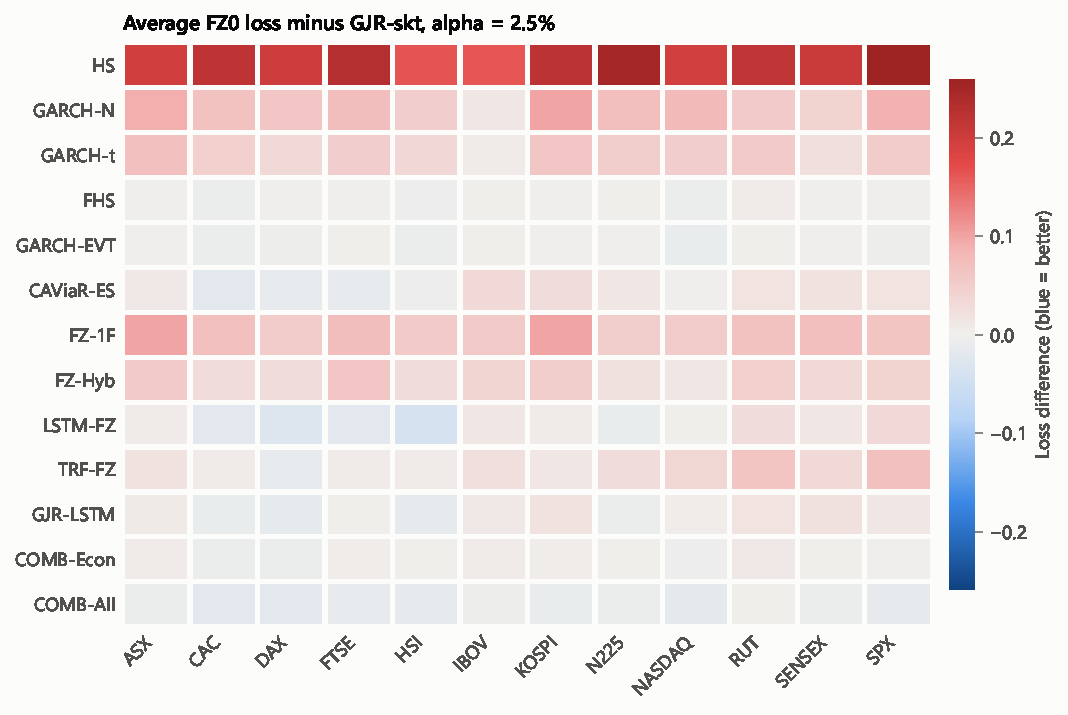
\includegraphics[width=\textwidth]{figures/heatmap_a025.pdf}
\caption{Average FZ0 loss difference from GJR-skt by asset, $\alpha=2.5\%$ (blue: lower loss).}\label{fig:heatmap}
\end{figure}

\subsection{Do the deep models add information?}
The cleanest test compares the two pre-specified combinations, which differ only in whether the three deep models are included. Table~\ref{tab:combo} shows that adding them lowers the loss at every risk level, with panel DM statistics between $-4.7$ and $-5.3$. The improvement is significant in 10 or 11 of the 12 markets and is never significantly negative. Figure~\ref{fig:combo} shows that the gain accumulates steadily over twenty years. It is not driven by a single episode: it is present before, during and after the global financial crisis and through the calm 2013--2019 period. A large part also comes after the COVID-19 shock. The deep models therefore contain information about tail risk that the econometric models, even averaged together, do not. This is our main finding. On their own the networks only match the best benchmarks, but they are \emph{complementary} to them.

\begin{table}[htbp]
\centering
\footnotesize
\caption{Value of adding the deep models to an econometric forecast combination}
\label{tab:combo}
\begin{tabular}{lrrrrr}
\toprule
Level & Loss diff & Panel DM t & p-value & \# assets better & \# assets worse \\
\midrule
1\% & -0.0168 & -4.73 & 0.000 & 10 & 0 \\
2.5\% & -0.0108 & -4.99 & 0.000 & 10 & 0 \\
5\% & -0.0080 & -5.25 & 0.000 & 11 & 0 \\
\bottomrule
\end{tabular}
\par\smallskip\parbox{\linewidth}{\scriptsize Loss difference COMB-All minus COMB-Econ (negative = adding the three deep models helps). The two combinations were specified before any results were seen and differ only by the inclusion of the deep models.}
\end{table}

\begin{figure}[htbp]\centering
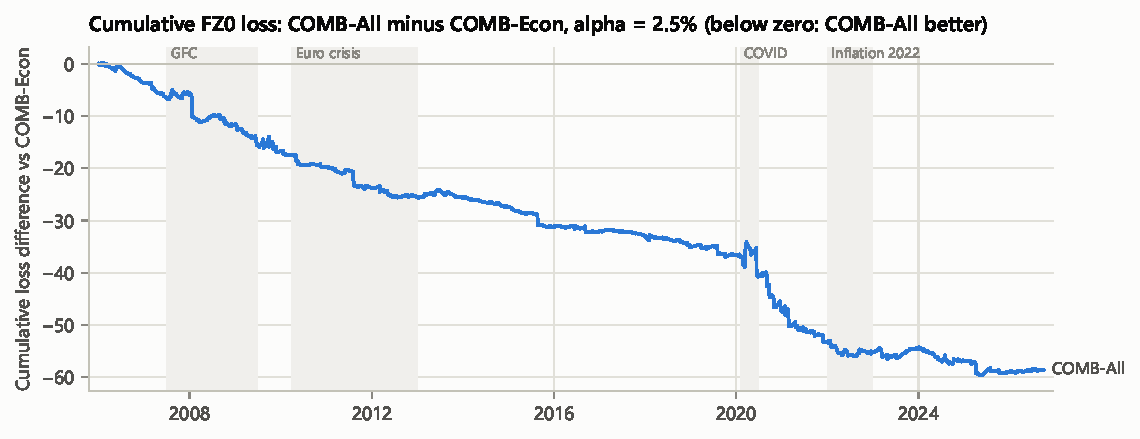
\includegraphics[width=\textwidth]{figures/cumulative_combo.pdf}
\caption{Cumulative FZ0 loss of COMB-All minus COMB-Econ (cross-asset average), $\alpha=2.5\%$. A downward slope means that adding the deep models to the combination lowers the loss.}\label{fig:combo}
\end{figure}

\subsection{Model confidence sets}
Table~\ref{tab:mcs} confirms the ranking. LSTM-FZ is the only single model contained in the 90\% MCS for all 36 asset--level combinations, and COMB-All is the only model in the pooled MCS with $p=1$ at every level. At $2.5\%$ the pooled MCS is $\{$COMB-All, LSTM-FZ, GJR-skt, FHS, GARCH-EVT$\}$. COMB-Econ has essentially the same average loss as GJR-skt yet is excluded from every pooled MCS. The reason is that its loss differential to COMB-All is small but extremely stable, so it is estimated very precisely.

\begin{table}[htbp]
\centering
\footnotesize
\caption{Model confidence set (90\%) membership}
\label{tab:mcs}
\resizebox{\textwidth}{!}{%
\begin{tabular}{lrrrrrr}
\toprule
Model & \# assets 1\% & \# assets 2.5\% & \# assets 5\% & Pooled p 1\% & Pooled p 2.5\% & Pooled p 5\% \\
\midrule
HS & 0 & 0 & 0 & 0.001 & 0.001 & 0.000 \\
GARCH-N & 1 & 1 & 1 & 0.001 & 0.000 & 0.000 \\
GARCH-t & 5 & 2 & 1 & 0.001 & 0.000 & 0.000 \\
GJR-skt & 12 & 11 & 11 & 0.299 & 0.166 & 0.328 \\
FHS & 12 & 11 & 11 & 0.169 & 0.174 & 0.281 \\
GARCH-EVT & 12 & 11 & 12 & 0.348 & 0.174 & 0.328 \\
CAViaR-ES & 12 & 12 & 11 & 0.009 & 0.035 & 0.328 \\
FZ-1F & 2 & 0 & 0 & 0.000 & 0.000 & 0.000 \\
FZ-Hyb & 6 & 1 & 0 & 0.005 & 0.000 & 0.000 \\
LSTM-FZ & 12 & 12 & 12 & 0.528 & 0.406 & 0.328 \\
TRF-FZ & 12 & 11 & 9 & 0.183 & 0.048 & 0.044 \\
GJR-LSTM & 12 & 10 & 12 & 0.057 & 0.035 & 0.126 \\
COMB-Econ & 8 & 6 & 5 & 0.001 & 0.000 & 0.000 \\
COMB-All & 12 & 12 & 12 & 1.000 & 1.000 & 1.000 \\
\bottomrule
\end{tabular}
}
\par\smallskip\parbox{\linewidth}{\scriptsize Columns '\# assets': number of assets whose MCS contains the model. 'Pooled p': MCS p-value on the cross-asset average loss series; a model is in the pooled MCS if p > 0.1. Range statistic, stationary bootstrap, 2000 replications.}
\end{table}

\subsection{Calibration}
Table~\ref{tab:bt_a025} reports absolute backtests. Accuracy and calibration rank models differently. GARCH-EVT and FHS are the best-calibrated models: their violation rates are within 0.1 percentage points of nominal, and they are rarely rejected by any VaR or ES test. The deep models are slightly less conservative, with violation rates of 2.79--2.80\% at the 2.5\% level. They are rejected more often by the coverage and calibration tests, and the Transformer is rejected by the dynamic-quantile test in all twelve markets. This indicates that its forecasts react too slowly to new information. All models have negative Acerbi--Szekely $Z_2$, i.e.\ a slight tendency to understate ES. The tendency is smallest for GARCH-EVT, FHS and COMB-All. COMB-All has a violation rate of 2.67\% and is rejected by the unconditional and conditional coverage tests in no market. The combination therefore inherits the accuracy of the deep models without their calibration weaknesses.

\begin{table}[htbp]
\centering
\footnotesize
\caption{Backtests, $\alpha=0.025$: number of assets (out of 12) rejecting at 5\%}
\label{tab:bt_a025}
\begin{tabular}{lrrrrrrrr}
\toprule
Model & Hit \% & UC & CC & DQ & ER & CCT-u & CCT-c & Z2 \\
\midrule
HS & 3.20 & 11 & 12 & 12 & 12 & 12 & 12 & -0.400 \\
GARCH-N & 3.68 & 11 & 11 & 12 & 12 & 12 & 12 & -0.652 \\
GARCH-t & 3.51 & 11 & 11 & 11 & 6 & 11 & 11 & -0.454 \\
GJR-skt & 2.72 & 2 & 3 & 3 & 2 & 2 & 3 & -0.114 \\
FHS & 2.60 & 0 & 1 & 1 & 2 & 0 & 0 & -0.067 \\
GARCH-EVT & 2.58 & 0 & 1 & 1 & 1 & 0 & 1 & -0.051 \\
CAViaR-ES & 2.73 & 3 & 2 & 5 & 5 & 4 & 1 & -0.133 \\
FZ-1F & 2.74 & 3 & 2 & 6 & 4 & 4 & 7 & -0.129 \\
FZ-Hyb & 2.74 & 2 & 2 & 3 & 5 & 5 & 2 & -0.135 \\
LSTM-FZ & 2.80 & 5 & 3 & 5 & 4 & 4 & 5 & -0.143 \\
TRF-FZ & 2.79 & 2 & 3 & 12 & 8 & 6 & 4 & -0.170 \\
GJR-LSTM & 2.79 & 5 & 6 & 6 & 4 & 5 & 4 & -0.155 \\
COMB-Econ & 2.78 & 4 & 3 & 4 & 3 & 3 & 3 & -0.143 \\
COMB-All & 2.67 & 0 & 0 & 4 & 4 & 1 & 3 & -0.095 \\
\bottomrule
\end{tabular}
\par\smallskip\parbox{\linewidth}{\scriptsize Hit \%: average violation rate (nominal 2.5\%). VaR tests: UC Kupiec, CC Christoffersen conditional coverage, DQ Engle--Manganelli. ES tests: ER McNeil--Frey exceedance residuals (one-sided bootstrap), CCT-u/CCT-c Nolde--Ziegel unconditional/conditional calibration. Z2: Acerbi--Szekely statistic averaged over assets (negative = ES too optimistic).}
\end{table}

\subsection{Crisis periods}
Table~\ref{tab:sub} and Figure~\ref{fig:cumdiff} show where the deep models gain and lose. LSTM-FZ accumulates a steady advantage over GJR-skt in calm and moderately volatile periods (2013--2019 and the euro-area crisis), and gives much of it back in a few days in March 2020. The COVID-19 crash was the fastest volatility increase in the sample, and GARCH-type recursions, which react to every squared return, adapted faster than networks trained on the previous eight years. The Transformer has its two largest losses in February 2018 (``Volmageddon'') and March 2020, both sudden volatility spikes. The hybrid, whose scale comes from GARCH, loses far less in March 2020 (0.12 against 0.35 for LSTM-FZ). None of the deep models' or combinations' crisis-period differences is significant at 5\%, because these windows are short. Figure~\ref{fig:episodes} illustrates the forecasts during the global financial crisis and the COVID-19 crash.

\begin{table}[htbp]
\centering
\footnotesize
\caption{Loss difference vs GJR-skt by subperiod, $\alpha=0.025$}
\label{tab:sub}
\begin{tabular}{lrrrrr}
\toprule
 & GFC & Euro crisis & COVID & Inflation 2022 & Calm 2013-2019 \\
\midrule
HS & 0.417 (3.3) & 0.278 (2.8) & 1.854 (1.6) & 0.170 (2.1) & 0.106 (2.7) \\
GARCH-N & 0.112 (2.5) & 0.056 (1.6) & 0.514 (1.6) & 0.106 (2.2) & 0.050 (2.6) \\
GARCH-t & 0.088 (2.3) & 0.048 (1.6) & 0.312 (1.3) & 0.064 (2.0) & 0.032 (2.2) \\
FHS & 0.005 (1.0) & -0.001 (-0.4) & -0.016 (-0.6) & -0.004 (-0.8) & 0.001 (0.5) \\
GARCH-EVT & 0.000 (0.0) & -0.001 (-0.3) & -0.012 (-0.4) & -0.005 (-0.9) & 0.002 (0.7) \\
CAViaR-ES & 0.037 (1.6) & 0.010 (1.3) & 0.264 (1.5) & -0.002 (-0.1) & -0.007 (-1.0) \\
FZ-1F & 0.096 (3.7) & 0.068 (3.4) & 0.457 (1.6) & 0.083 (2.7) & 0.056 (4.3) \\
FZ-Hyb & 0.073 (2.9) & 0.025 (1.7) & 0.406 (1.3) & 0.035 (1.3) & 0.033 (3.2) \\
LSTM-FZ & 0.013 (0.4) & -0.018 (-1.3) & 0.351 (0.9) & 0.011 (0.3) & -0.012 (-1.4) \\
TRF-FZ & 0.023 (0.7) & -0.001 (-0.1) & 0.626 (1.0) & 0.054 (1.6) & 0.016 (0.9) \\
GJR-LSTM & 0.039 (1.7) & 0.001 (0.2) & 0.121 (0.7) & 0.043 (1.4) & -0.004 (-0.8) \\
COMB-Econ & 0.009 (0.8) & 0.004 (0.5) & 0.110 (0.9) & -0.003 (-0.3) & 0.001 (0.2) \\
COMB-All & -0.008 (-0.9) & -0.007 (-0.8) & 0.072 (0.4) & -0.011 (-0.9) & -0.005 (-1.1) \\
\bottomrule
\end{tabular}
\par\smallskip\parbox{\linewidth}{\scriptsize Average FZ0 loss difference (negative = better than the benchmark); panel Diebold--Mariano t-statistic in parentheses.}
\end{table}

\begin{figure}[htbp]\centering
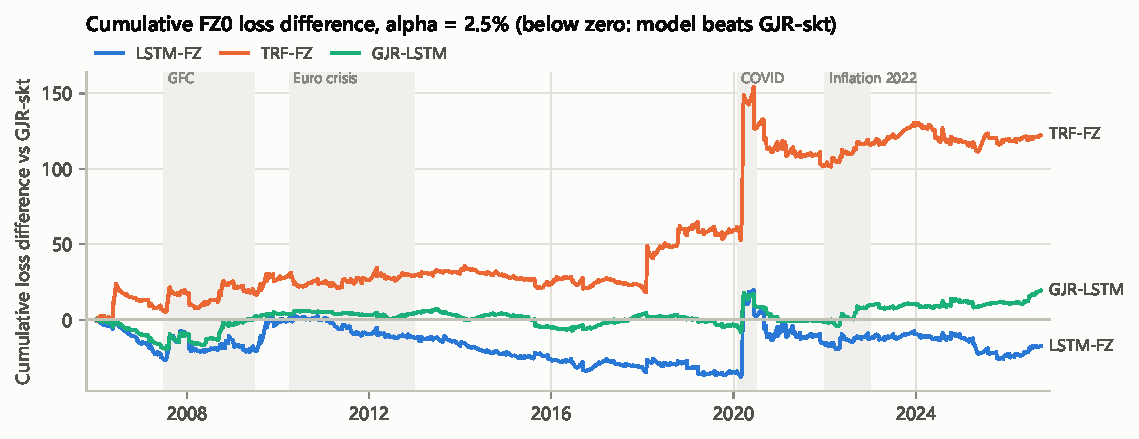
\includegraphics[width=\textwidth]{figures/cumulative_diff.pdf}
\caption{Cumulative FZ0 loss of each deep model minus GJR-skt (cross-asset average), $\alpha=2.5\%$. Shaded: crisis subperiods.}\label{fig:cumdiff}
\end{figure}

\begin{figure}[htbp]\centering
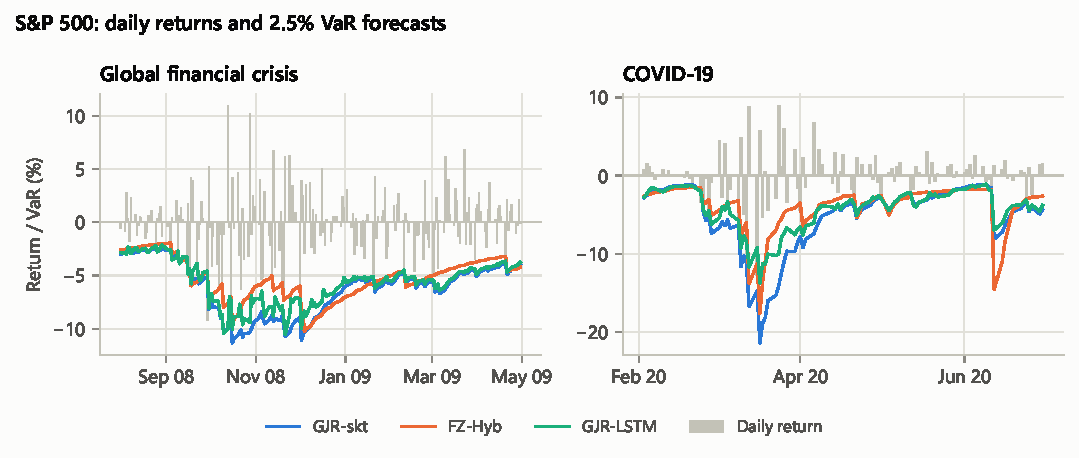
\includegraphics[width=\textwidth]{figures/episodes.pdf}
\caption{S\&P 500 daily returns and 2.5\% VaR forecasts of GJR-skt, FZ-Hyb and GJR-LSTM during the global financial crisis and the COVID-19 crash.}\label{fig:episodes}
\end{figure}

\subsection{A regulatory view}
Table~\ref{tab:reg} translates forecasts into the two quantities a bank cares about. The first is the level of the 97.5\% ES, the FRTB capital measure. The second is the Basel traffic light for 99\% VaR backtesting. GARCH-EVT is the most conservative model: it has the highest average ES and the fewest days in the yellow and red zones. COMB-All requires 2.2\% less capital than GJR-skt (3.17\% against 3.24\% of position value). Its traffic-light record is essentially identical (16.9\% against 16.7\% of days in the yellow zone, 0.24\% against 0.26\% in the red zone). The individual deep models need similar or slightly less capital (3.15--3.19\%), but they spend 2.5--3 times as many days in the red zone as GJR-skt.

\begin{table}[htbp]
\centering
\footnotesize
\caption{Regulatory view: capital and Basel traffic light}
\label{tab:reg}
\begin{tabular}{lrrr}
\toprule
Model & Capital (avg -ES 2.5\%) & Yellow zone \% days & Red zone \% days \\
\midrule
HS & 3.41 & 36.3 & 5.7 \\
GARCH-N & 2.78 & 51.1 & 6.0 \\
GARCH-t & 3.06 & 37.4 & 1.3 \\
GJR-skt & 3.24 & 16.7 & 0.3 \\
FHS & 3.26 & 18.9 & 0.2 \\
GARCH-EVT & 3.28 & 13.6 & 0.1 \\
CAViaR-ES & 3.18 & 20.6 & 2.4 \\
FZ-1F & 3.33 & 20.5 & 2.1 \\
FZ-Hyb & 3.24 & 18.8 & 0.9 \\
LSTM-FZ & 3.19 & 19.0 & 0.7 \\
TRF-FZ & 3.18 & 23.4 & 0.8 \\
GJR-LSTM & 3.15 & 23.6 & 0.6 \\
COMB-Econ & 3.17 & 18.7 & 0.5 \\
COMB-All & 3.17 & 16.9 & 0.2 \\
\bottomrule
\end{tabular}
\par\smallskip\parbox{\linewidth}{\scriptsize Capital: average forecast of $-\mathrm{ES}_{2.5\%}$ (FRTB measure), in \% of position value, averaged over assets. Traffic light: share of days on which the trailing 250-day count of 99\% VaR violations is 5--9 (yellow) or $\geq$10 (red).}
\end{table}

\subsection{What does the hybrid learn?}
Figure~\ref{fig:tail} plots the ES/VaR ratio implied by each model, a scale-free measure of tail heaviness. In GARCH-$t$ and GJR-skt it moves only through re-estimated shape parameters. Over 2006--2026 these drift upward from 1.25 to 1.35, as the rolling window absorbs more crash days. The hybrid's ratio is far more variable. It falls well below the parametric ratios during the calm 2012--2019 period, which means thinner standardised tails than the skewed-$t$ implies. It rises sharply after 2020 and stays above them during 2023--2024. The network therefore learns economically interpretable variation in tail shape. That this variation does not translate into significantly better forecasts suggests that, at a daily horizon and with returns alone, the predictable component of tail shape beyond volatility is small.

\begin{figure}[htbp]\centering
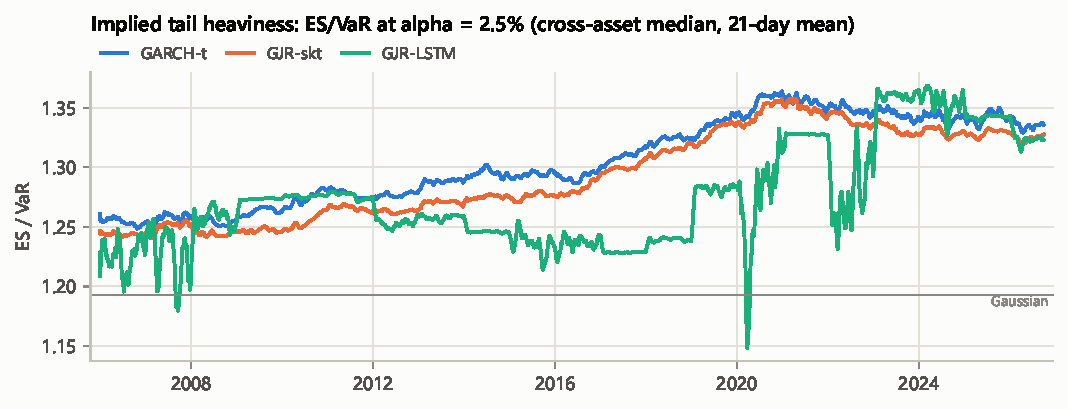
\includegraphics[width=\textwidth]{figures/tail_ratio.pdf}
\caption{Model-implied ES/VaR at $\alpha=2.5\%$ (cross-asset median, 21-day moving average). The grey line is the Gaussian value 1.193.}\label{fig:tail}
\end{figure}

\subsection{Robustness}
\paragraph{Seeds.} Table~\ref{tab:seeds} compares single networks with the three-seed ensembles. For LSTM-FZ, average losses across seeds differ by up to 0.007. That is larger than the differences among the four best models, so comparisons based on a single trained network would be unreliable. The ensemble is better than every individual seed for LSTM-FZ, and better than all but one for the other two models.

\paragraph{Specification revisions.} Two choices were revised after the first full run: the initialisation of the networks' output head and the optimiser for the semiparametric models (Appendix~\ref{app:v1}). Neither revision changes any conclusion. COMB-All is best, LSTM-FZ matches the top econometric models, and the FZ-GAS models underperform in both runs.

\begin{table}[htbp]
\centering
\footnotesize
\caption{Deep models: single seeds versus the seed ensemble, $\alpha=0.025$}
\label{tab:seeds}
\begin{tabular}{lrrrr}
\toprule
Model & Ensemble & Seed 0 & Seed 1 & Seed 2 \\
\midrule
GJR-LSTM & 1.1300 & 1.1336 & 1.1306 & 1.1297 \\
LSTM-FZ & 1.1244 & 1.1261 & 1.1251 & 1.1317 \\
TRF-FZ & 1.1497 & 1.1459 & 1.1656 & 1.1528 \\
\bottomrule
\end{tabular}
\end{table}


%==============================================================================
\section{Conclusion}\label{sec:conclusion}
%==============================================================================
Because (VaR, ES) is jointly elicitable, a neural network can be trained to forecast Expected Shortfall in exactly the way it is evaluated, by minimising a strictly consistent scoring function. We derived the properties that make this practical. Pooling across markets is exact under scale standardisation, and an output layer can guarantee coherent, non-crossing forecasts. We then evaluated the approach against a demanding set of benchmarks over twenty years and twelve markets.

Three conclusions follow. First, a pooled LSTM trained on FZ0 matches, but does not beat, the best econometric models (GJR-GARCH with skewed-$t$ innovations, filtered historical simulation and GARCH-EVT). Second, the deep models carry information that the econometric models do not. Adding them to an econometric forecast combination improves accuracy at every risk level, in almost every market and steadily over time. The result is the best model in our study and a modest saving in regulatory capital at an unchanged backtesting record. Third, the networks' weaknesses are specific and interpretable. They are slightly less conservative than the best econometric models and are slower to adapt to unprecedented volatility spikes. A hybrid that takes its volatility scale from GARCH mitigates the second weakness but learns little that improves forecasts. This suggests that, from daily returns alone, the predictable variation in tail shape beyond volatility is small.

\paragraph{Limitations.} The information set is deliberately restricted to daily returns, the horizon is one day, and the study covers equity indices only. Hyperparameters were fixed in advance rather than tuned. Two implementation choices were revised after a first run, both transparently documented and neither affecting the conclusions. The calibration test we use is mildly oversized in samples of the size of a single market's history.

\paragraph{Extensions.} Natural next steps include adding realised measures or intraday ranges to separate the value of information from that of architecture, multi-day horizons, and robustness of the ranking across the whole class of consistent scoring functions via Murphy diagrams \citep{ziegel2020robust}. The most interesting extension is economic: whether the time-varying tail shape learned by the hybrid is priced in the cross-section or predicts market returns, in the spirit of \citet{kelly2014tail}.


\section*{Acknowledgments and disclosure}
The author used AI-based assistance (large language model tools) for code development, literature search and editing. All modelling choices, results and interpretations were checked by the author, who takes full responsibility for the content of this paper. Any errors are the author's own.

\bibliographystyle{plainnat}
\bibliography{references}

\appendix
\section{Hyperparameters and implementation}\label{app:hyper}
\begin{table}[htbp]\centering\footnotesize
\caption{Deep-model hyperparameters (fixed ex ante)}
\begin{tabular}{ll}\toprule
Input length $L$ & 64 trading days \\
Slow scale window & 250 days \\
Hidden size / layers & 32 / 1 (LSTM); 32 / 1 layer, 2 heads (Transformer) \\
Head & MLP 32 units, GELU, dropout 0.1, monotone output \eqref{eq:head} \\
Optimiser & AdamW, learning rate $10^{-3}$, weight decay $10^{-4}$, batch 512, gradient clip 1 \\
Early stopping & patience 8 epochs (maximum 60) on the last 20\% of each training window \\
Training sample & pooled across 12 assets, last 2000 days each ($\approx$24{,}000 sequences) \\
Re-training & yearly; 3 seeds averaged \\
\bottomrule\end{tabular}
\end{table}
All code is in Python (\texttt{numpy}, \texttt{arch}, \texttt{numba}, \texttt{PyTorch}). The full pipeline (data download, forecasting, evaluation, tables and figures) runs from four scripts. Unit tests cover the strict consistency of the loss, the size of every backtest under the null, alignment with the \texttt{arch} package, and the absence of look-ahead for every model.

\section{Additional tables}
\begin{table}[htbp]
\centering
\footnotesize
\caption{Average FZ0 loss, $\alpha=0.01$}
\label{tab:loss_a010}
\begin{tabular}{lrrrrrr}
\toprule
Model & Avg loss & Diff vs bench & Panel DM t & \# better & \# worse & Mean rank \\
\midrule
HS & 1.6353 & 0.3002 & 4.46 & 0 & 12 & 14.0 \\
GARCH-N & 1.4708 & 0.1372 & 4.74 & 0 & 10 & 12.2 \\
GARCH-t & 1.3828 & 0.0496 & 2.96 & 0 & 5 & 9.5 \\
GJR-skt & 1.3351 & 0.0000 &  & 0 & 0 & 5.2 \\
FHS & 1.3355 & 0.0008 & 0.27 & 0 & 1 & 5.4 \\
GARCH-EVT & 1.3304 & -0.0043 & -1.40 & 0 & 0 & 3.5 \\
CAViaR-ES & 1.3565 & 0.0220 & 1.57 & 0 & 0 & 7.7 \\
FZ-1F & 1.4490 & 0.1201 & 5.28 & 0 & 10 & 11.8 \\
FZ-Hyb & 1.4173 & 0.0848 & 2.75 & 0 & 5 & 10.8 \\
LSTM-FZ & 1.3281 & -0.0082 & -0.45 & 0 & 0 & 3.8 \\
TRF-FZ & 1.3616 & 0.0246 & 0.83 & 0 & 0 & 8.2 \\
GJR-LSTM & 1.3414 & 0.0062 & 0.62 & 0 & 0 & 5.8 \\
COMB-Econ & 1.3346 & 0.0015 & 0.17 & 0 & 0 & 5.1 \\
COMB-All & \textbf{1.3185} & -0.0153 & -1.65 & 0 & 0 & \textbf{2.1} \\
\bottomrule
\end{tabular}
\par\smallskip\parbox{\linewidth}{\scriptsize Avg loss: FZ0 loss averaged over days and then over the 12 assets. Diff vs bench: average loss minus that of GJR-skt (negative = better); Panel DM t: Diebold--Mariano statistic on the cross-asset average loss differential (Newey--West). \# better / worse: assets where the single-asset DM test is significant at 5\%. Mean rank across assets (1 = best).}
\end{table}
\begin{table}[htbp]
\centering
\footnotesize
\caption{Average FZ0 loss, $\alpha=0.05$}
\label{tab:loss_a050}
\begin{tabular}{lrrrrrr}
\toprule
Model & Avg loss & Diff vs bench & Panel DM t & \# better & \# worse & Mean rank \\
\midrule
HS & 1.1063 & 0.1599 & 5.45 & 0 & 12 & 14.0 \\
GARCH-N & 0.9829 & 0.0359 & 4.60 & 0 & 11 & 11.7 \\
GARCH-t & 0.9808 & 0.0338 & 4.48 & 0 & 10 & 10.8 \\
GJR-skt & 0.9469 & 0.0000 &  & 0 & 0 & 4.3 \\
FHS & 0.9461 & -0.0004 & -0.35 & 1 & 0 & 4.1 \\
GARCH-EVT & 0.9458 & -0.0008 & -0.71 & 1 & 0 & 3.8 \\
CAViaR-ES & 0.9485 & 0.0012 & 0.35 & 1 & 0 & 5.3 \\
FZ-1F & 0.9832 & 0.0367 & 6.86 & 0 & 12 & 11.7 \\
FZ-Hyb & 0.9713 & 0.0243 & 4.82 & 0 & 9 & 10.1 \\
LSTM-FZ & 0.9527 & 0.0047 & 0.53 & 0 & 0 & 6.0 \\
TRF-FZ & 0.9705 & 0.0228 & 1.84 & 0 & 3 & 10.2 \\
GJR-LSTM & 0.9494 & 0.0025 & 0.62 & 0 & 1 & 5.2 \\
COMB-Econ & 0.9494 & 0.0027 & 1.05 & 0 & 1 & 6.2 \\
COMB-All & \textbf{0.9415} & -0.0053 & -1.58 & 1 & 0 & \textbf{1.6} \\
\bottomrule
\end{tabular}
\par\smallskip\parbox{\linewidth}{\scriptsize Avg loss: FZ0 loss averaged over days and then over the 12 assets. Diff vs bench: average loss minus that of GJR-skt (negative = better); Panel DM t: Diebold--Mariano statistic on the cross-asset average loss differential (Newey--West). \# better / worse: assets where the single-asset DM test is significant at 5\%. Mean rank across assets (1 = best).}
\end{table}
\begin{table}[htbp]
\centering
\footnotesize
\caption{Backtests, $\alpha=0.01$: number of assets (out of 12) rejecting at 5\%}
\label{tab:bt_a010}
\begin{tabular}{lrrrrrrrr}
\toprule
Model & Hit \% & UC & CC & DQ & ER & CCT-u & CCT-c & Z2 \\
\midrule
HS & 1.70 & 12 & 12 & 12 & 12 & 12 & 12 & -0.883 \\
GARCH-N & 2.06 & 12 & 12 & 12 & 12 & 12 & 12 & -1.324 \\
GARCH-t & 1.60 & 11 & 11 & 12 & 2 & 9 & 9 & -0.644 \\
GJR-skt & 1.13 & 0 & 2 & 5 & 3 & 1 & 1 & -0.169 \\
FHS & 1.14 & 2 & 3 & 6 & 1 & 1 & 0 & -0.173 \\
GARCH-EVT & 1.03 & 0 & 1 & 3 & 3 & 1 & 1 & -0.072 \\
CAViaR-ES & 1.21 & 4 & 4 & 5 & 6 & 4 & 2 & -0.276 \\
FZ-1F & 1.28 & 7 & 5 & 8 & 4 & 7 & 10 & -0.331 \\
FZ-Hyb & 1.21 & 4 & 4 & 6 & 10 & 8 & 3 & -0.307 \\
LSTM-FZ & 1.14 & 5 & 4 & 8 & 2 & 3 & 2 & -0.170 \\
TRF-FZ & 1.29 & 6 & 6 & 10 & 4 & 5 & 5 & -0.348 \\
GJR-LSTM & 1.25 & 5 & 6 & 6 & 4 & 5 & 3 & -0.290 \\
COMB-Econ & 1.18 & 3 & 2 & 6 & 5 & 2 & 0 & -0.227 \\
COMB-All & 1.13 & 1 & 2 & 6 & 2 & 0 & 0 & -0.166 \\
\bottomrule
\end{tabular}
\par\smallskip\parbox{\linewidth}{\scriptsize Hit \%: average violation rate (nominal 1\%). VaR tests: UC Kupiec, CC Christoffersen conditional coverage, DQ Engle--Manganelli. ES tests: ER McNeil--Frey exceedance residuals (one-sided bootstrap), CCT-u/CCT-c Nolde--Ziegel unconditional/conditional calibration. Z2: Acerbi--Szekely statistic averaged over assets (negative = ES too optimistic).}
\end{table}
\begin{table}[htbp]
\centering
\footnotesize
\caption{Backtests, $\alpha=0.05$: number of assets (out of 12) rejecting at 5\%}
\label{tab:bt_a050}
\begin{tabular}{lrrrrrrrr}
\toprule
Model & Hit \% & UC & CC & DQ & ER & CCT-u & CCT-c & Z2 \\
\midrule
HS & 5.66 & 9 & 11 & 12 & 12 & 12 & 12 & -0.215 \\
GARCH-N & 5.91 & 9 & 9 & 10 & 12 & 12 & 12 & -0.325 \\
GARCH-t & 6.30 & 11 & 11 & 12 & 8 & 11 & 12 & -0.315 \\
GJR-skt & 5.23 & 2 & 1 & 3 & 4 & 1 & 5 & -0.068 \\
FHS & 5.02 & 0 & 1 & 2 & 4 & 0 & 4 & -0.024 \\
GARCH-EVT & 5.08 & 0 & 1 & 3 & 2 & 0 & 3 & -0.030 \\
CAViaR-ES & 5.10 & 0 & 1 & 4 & 5 & 1 & 4 & -0.052 \\
FZ-1F & 5.12 & 0 & 2 & 1 & 4 & 3 & 8 & -0.045 \\
FZ-Hyb & 5.13 & 0 & 1 & 2 & 4 & 3 & 4 & -0.056 \\
LSTM-FZ & 5.65 & 9 & 9 & 8 & 1 & 8 & 8 & -0.138 \\
TRF-FZ & 5.25 & 1 & 2 & 11 & 8 & 5 & 6 & -0.090 \\
GJR-LSTM & 5.18 & 1 & 3 & 2 & 8 & 4 & 4 & -0.072 \\
COMB-Econ & 5.23 & 1 & 2 & 4 & 6 & 4 & 6 & -0.077 \\
COMB-All & 5.18 & 0 & 2 & 3 & 3 & 0 & 2 & -0.058 \\
\bottomrule
\end{tabular}
\par\smallskip\parbox{\linewidth}{\scriptsize Hit \%: average violation rate (nominal 5\%). VaR tests: UC Kupiec, CC Christoffersen conditional coverage, DQ Engle--Manganelli. ES tests: ER McNeil--Frey exceedance residuals (one-sided bootstrap), CCT-u/CCT-c Nolde--Ziegel unconditional/conditional calibration. Z2: Acerbi--Szekely statistic averaged over assets (negative = ES too optimistic).}
\end{table}
\begin{table}[htbp]
\centering
\footnotesize
\caption{Average FZ0 loss by asset, $\alpha=0.025$: level for GJR-skt, difference for every other model}
\label{tab:perasset}
\resizebox{\textwidth}{!}{%
\begin{tabular}{lrrrrrrrrrrrrrr}
\toprule
Asset & GJR-skt (level) & HS & GARCH-N & GARCH-t & FHS & GARCH-EVT & CAViaR-ES & FZ-1F & FZ-Hyb & LSTM-FZ & TRF-FZ & GJR-LSTM & COMB-Econ & COMB-All \\
\midrule
ASX & 0.901 & 0.196 & 0.090 & 0.068 & -0.002 & -0.002 & 0.009 & 0.098 & 0.053 & 0.004 & 0.019 & 0.007 & 0.006 & -0.007 \\
CAC & 1.135 & 0.219 & 0.066 & 0.045 & -0.006 & -0.006 & -0.020 & 0.067 & 0.027 & -0.019 & 0.005 & -0.010 & -0.008 & -0.019 \\
DAX & 1.135 & 0.198 & 0.059 & 0.032 & -0.002 & -0.004 & -0.012 & 0.051 & 0.028 & -0.028 & -0.011 & -0.016 & -0.007 & -0.020 \\
FTSE & 0.927 & 0.231 & 0.072 & 0.048 & -0.001 & 0.000 & -0.012 & 0.072 & 0.060 & -0.019 & 0.004 & 0.002 & 0.004 & -0.010 \\
HSI & 1.235 & 0.163 & 0.048 & 0.033 & -0.006 & -0.007 & -0.006 & 0.055 & 0.025 & -0.037 & 0.005 & -0.013 & 0.001 & -0.013 \\
IBOV & 1.306 & 0.162 & 0.011 & 0.004 & 0.002 & 0.002 & 0.032 & 0.057 & 0.037 & 0.012 & 0.024 & 0.009 & 0.005 & -0.003 \\
KOSPI & 1.125 & 0.220 & 0.099 & 0.059 & -0.001 & -0.001 & 0.026 & 0.099 & 0.050 & 0.006 & 0.013 & 0.020 & 0.003 & -0.008 \\
N225 & 1.267 & 0.248 & 0.071 & 0.050 & 0.000 & -0.001 & 0.013 & 0.049 & 0.021 & -0.010 & 0.026 & -0.006 & 0.000 & -0.008 \\
NASDAQ & 1.198 & 0.194 & 0.078 & 0.049 & -0.007 & -0.008 & -0.001 & 0.051 & 0.013 & 0.000 & 0.036 & 0.004 & -0.006 & -0.017 \\
RUT & 1.242 & 0.216 & 0.054 & 0.054 & 0.005 & 0.002 & 0.018 & 0.065 & 0.046 & 0.025 & 0.061 & 0.017 & 0.009 & 0.001 \\
SENSEX & 1.031 & 0.203 & 0.041 & 0.024 & -0.002 & -0.001 & 0.018 & 0.069 & 0.032 & 0.011 & 0.031 & 0.021 & 0.001 & -0.006 \\
SPX & 1.012 & 0.260 & 0.089 & 0.051 & -0.001 & -0.004 & 0.017 & 0.063 & 0.041 & 0.031 & 0.069 & 0.012 & -0.001 & -0.012 \\
\bottomrule
\end{tabular}
}
\par\smallskip\parbox{\linewidth}{\scriptsize Negative differences = lower loss than the benchmark.}
\end{table}
\clearpage


\section{First-run specification and revisions}\label{app:v1}
After the first complete run (v1) we made two changes. Both are documented here because they were made after out-of-sample results had been computed.

\paragraph{Initialisation of the deep models' output head.} In v1 the last-layer bias was set to standard-normal values of (VaR, ES). The training log showed that, for the GJR-LSTM hybrid, early stopping returned the untrained initial model for all three seeds in the 2014 and 2024 refits. Their validation windows (2012--2013 and 2022--2023) were calm, and no trained network improved on a thin Gaussian tail there. The hybrid therefore forecast with Gaussian standardised quantiles for those two years, which understates ES. The final specification initialises the head at the empirical (VaR, ES) of the pooled standardised training targets, so that the fallback is a historical-simulation tail. With this change six of 189 training jobs still fall back to their initial model, all for the hybrid and mostly in the 2009 refit, but the fallback is now an FHS-type model rather than a Gaussian one.

\paragraph{Estimation of the semiparametric models.} In v1, CAViaR-ES, FZ-1F and FZ-Hyb were estimated by Nelder--Mead from the best three points of a starting grid. Table~\ref{tab:estdiag} compares the resulting in-sample FZ0 loss ($\alpha=2.5\%$) with that of the final multi-start procedure and of a 300-start search followed by Nelder--Mead and Powell. The v1 procedure left gaps of up to 0.04, which is as large as FZ-1F's entire out-of-sample deficit. The final procedure is within about 0.01 of the intensive search and sometimes better. The last column reports GJR-skt's in-sample loss on the same windows. It is lower than the best FZ-1F fit in most windows, which shows that FZ-1F's underperformance is a feature of the model rather than of its estimation.

\begin{table}[htbp]\centering\footnotesize
\caption{Estimation quality: in-sample average FZ0 loss, $\alpha=2.5\%$, 2000-day window ending on the date shown}\label{tab:estdiag}
\begin{tabular}{llrrrrrrr}\toprule
& & \multicolumn{3}{c}{FZ-1F} & \multicolumn{3}{c}{FZ-Hyb} & GJR-skt \\
\cmidrule(lr){3-5}\cmidrule(lr){6-8}
Asset & Window end & v1 & final & 300-start & v1 & final & 300-start & \\ \midrule
SPX & 2008-01 & 0.9018 & 0.9018 & 0.9073 & 0.9170 & 0.9135 & 0.9047 & 0.8889 \\
SPX & 2015-01 & 1.1434 & 1.1137 & 1.1037 & 1.0856 & 1.0744 & 1.0721 & 1.0896 \\
SPX & 2020-01 & 0.8189 & 0.7791 & 0.7780 & 0.7904 & 0.7812 & 0.7791 & 0.7301 \\
DAX & 2008-01 & 1.1871 & 1.1798 & 1.1813 & 1.1516 & 1.1474 & 1.1477 & 1.1211 \\
DAX & 2015-01 & 1.2619 & 1.2432 & 1.2442 & 1.2246 & 1.2213 & 1.2149 & 1.2222 \\
DAX & 2020-01 & 1.0447 & 1.0448 & 1.0350 & 1.0112 & 1.0109 & 1.0097 & 1.0420 \\
SENSEX & 2008-01 & 1.3687 & 1.3481 & 1.3417 & 1.3513 & 1.3367 & 1.3352 & 1.3196 \\
SENSEX & 2015-01 & 1.2207 & 1.1983 & 1.2047 & 1.2080 & 1.2072 & 1.2085 & 1.1971 \\
SENSEX & 2020-01 & 0.7719 & 0.7686 & 0.7616 & 0.7748 & 0.7675 & 0.7652 & 0.7790 \\
\bottomrule\end{tabular}
\par\smallskip\parbox{\linewidth}{\scriptsize Cold-start fits on a single window. In the rolling exercise the estimators are also warm-started from the previous window's optimum.}
\end{table}

\paragraph{Effect on the results.} Table~\ref{tab:revisions} reports the loss difference from GJR-skt for every model affected by the revisions. The empirical initialisation improves LSTM-FZ and GJR-LSTM at the 1\% level, where the Gaussian fallback was most harmful. The stronger optimiser slightly \emph{raises} the out-of-sample loss of the FZ-GAS models despite their better in-sample fit, the usual signature of fitting noise in a non-smooth objective. No conclusion of the paper changes.

\begin{table}[htbp]
\centering
\footnotesize
\caption{First run (v1) versus final specification: FZ0 loss minus GJR-skt}
\label{tab:revisions}
\begin{tabular}{lrrrrrr}
\toprule
Model & v1 1\% & final 1\% & v1 2.5\% & final 2.5\% & v1 5\% & final 5\% \\
\midrule
CAViaR-ES & 0.0215 & 0.0220 & 0.0060 & 0.0060 & 0.0012 & 0.0012 \\
FZ-1F & 0.1135 & 0.1201 & 0.0627 & 0.0651 & 0.0343 & 0.0367 \\
FZ-Hyb & 0.0832 & 0.0848 & 0.0342 & 0.0377 & 0.0235 & 0.0243 \\
LSTM-FZ & 0.0018 & -0.0082 & -0.0014 & -0.0033 & 0.0042 & 0.0047 \\
TRF-FZ & 0.0200 & 0.0246 & 0.0163 & 0.0227 & 0.0174 & 0.0228 \\
GJR-LSTM & 0.0125 & 0.0062 & 0.0026 & 0.0036 & 0.0016 & 0.0025 \\
COMB-Econ & 0.0009 & 0.0015 & 0.0005 & 0.0007 & 0.0026 & 0.0027 \\
COMB-All & -0.0151 & -0.0153 & -0.0104 & -0.0102 & -0.0055 & -0.0053 \\
\bottomrule
\end{tabular}
\par\smallskip\parbox{\linewidth}{\scriptsize v1: Gaussian initialisation of the deep models' output head; grid + Nelder--Mead estimation of the semiparametric models. Final: empirical initialisation; multi-start + Powell estimation. Unchanged models are omitted. Negative = better than GJR-skt.}
\end{table}


\end{document}
